\section{Hardware}

\subsection{Board}

Board components are annotated in \Fref{fig:revision_f5}.
A detailed mechanical drawing describing the board dimensions is available in the Appendix. % TODO: Create reference

\vskip 2em

% \begin{figure}[H]
%     \centering
%     \begin{tikzpicture}[annotation/.style={circle, draw=black, fill=white, very thick, minimum size=7mm}]
%         \node at (0,0) {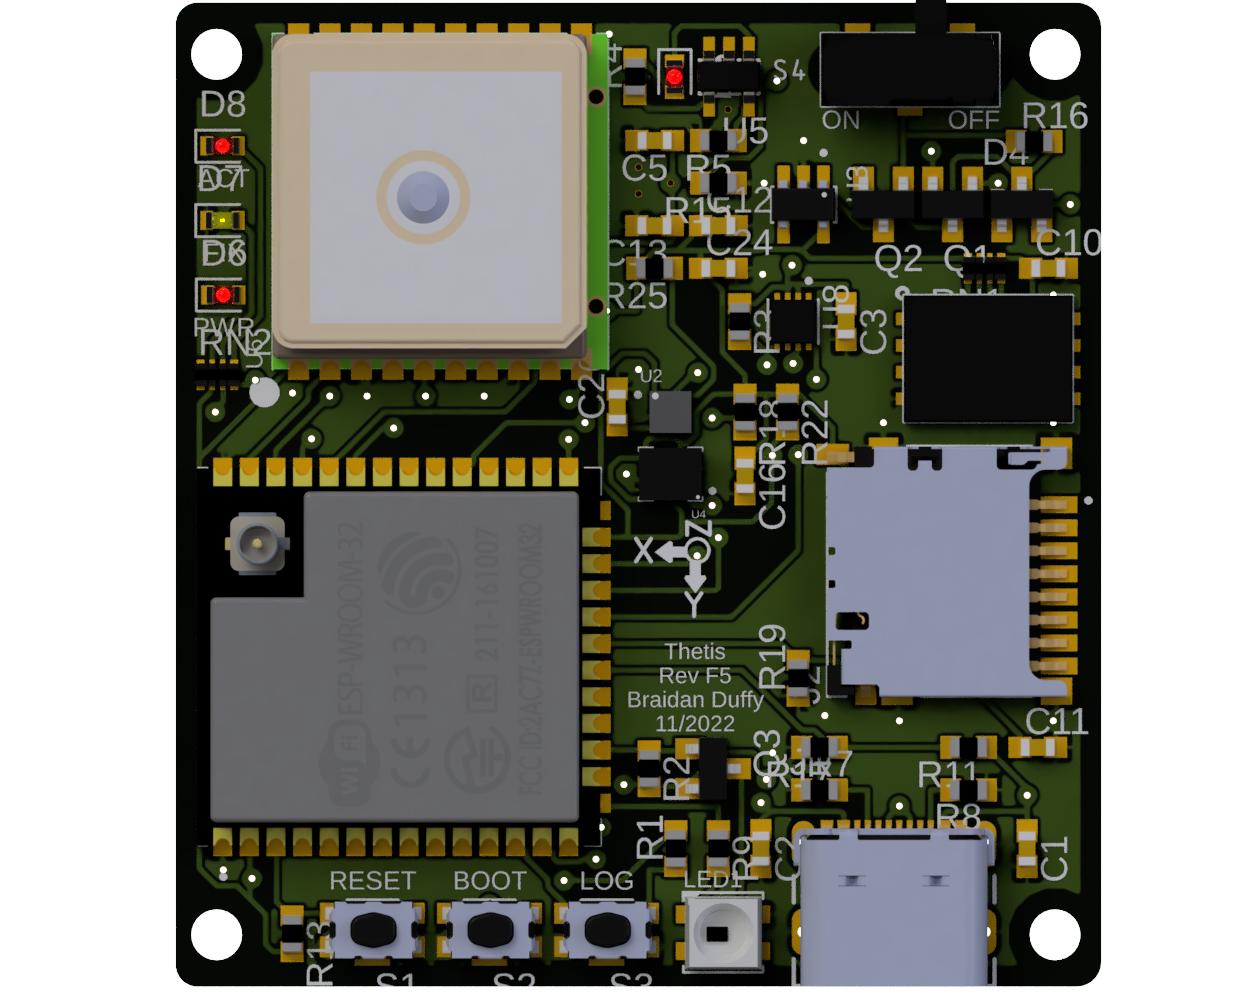
\includegraphics[width=0.95\textwidth]{Images/board.png}};
%         \node[annotation] at (-6,-4) {\ref{itm:board1}};
%         \node[annotation] at (-6.4,0) {\ref{itm:board2}};
%         \node[annotation] at (-5.7,3.7) {\ref{itm:board3}};
%         \node[annotation] at (-2.7,1.1) {\ref{itm:board4}};
%         \node[annotation] at (4.8,1.8) {\ref{itm:board5}};
%         \node[annotation] at (6.0,3.4) {\ref{itm:board6}};
%         \node[annotation] at (7.2,3.4) {\ref{itm:board7}};
%         \node[annotation] at (6.8,-1.9) {\ref{itm:board8}};
%         \node[annotation] at (5.5,-4) {\ref{itm:board9}};
%         \node[annotation] at (0.4,-0.8) {\ref{itm:board10}};
%         \node[annotation] at (-3.4,-2.9) {\ref{itm:board11}};
%     \end{tikzpicture}
%     \caption{Board}
%     \label{fig:board}
% \end{figure}

% \vskip 1em

% \begin{enumerate}
%     \item \label{itm:board1} Power button
%     \item \label{itm:board2} \acs{USB}-C connector
%     \item \label{itm:board3} \acs{LED}
%     \item \label{itm:board4} Serial header
%     \item \label{itm:board5} High-g accelerometer
%     \item \label{itm:board6} Inertial sensor (gyroscope and accelerometer)
%     \item \label{itm:board7} Magnetometer
%     \item \label{itm:board8} Wireless antennae
%     \item \label{itm:board9} U.FL connector for external wireless antennae
%     \item \label{itm:board10} \acs{microSD} socket
%     \item \label{itm:board11} Battery connector
% \end{enumerate}

\begin{figure}[h!]
    \centering
    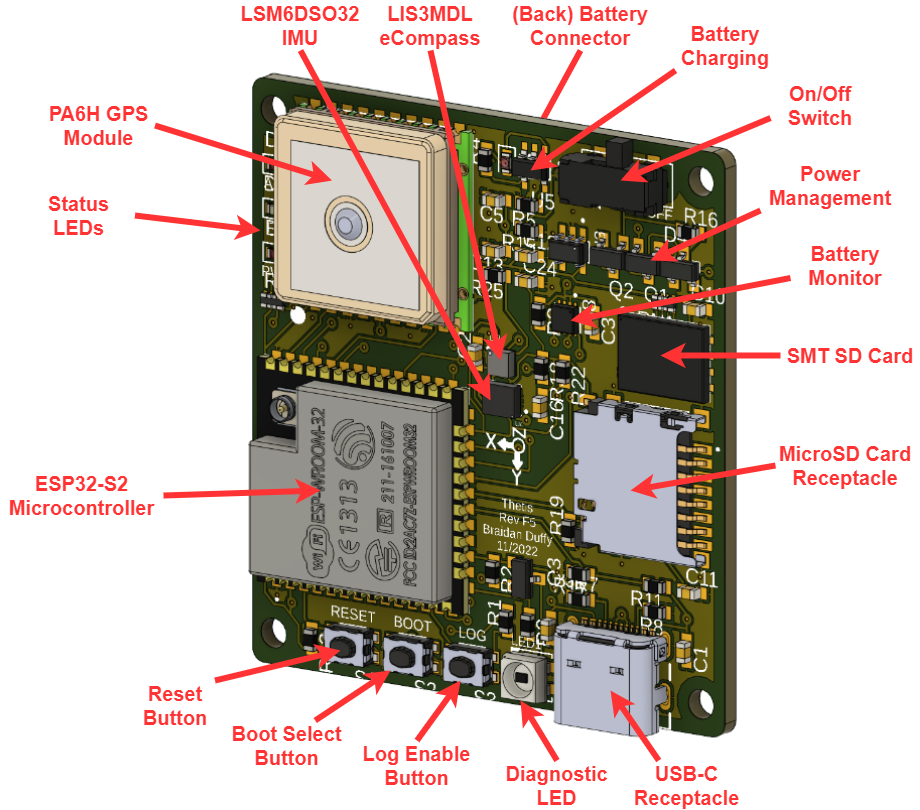
\includegraphics[width=\textwidth]{revision_f5_labeled.png}
    \caption{Revision F5 of Thetis with callouts for important components}
    \labfig{revision_f5}
\end{figure}

\clearpage

\subsubsection{Interface Pads}

The PCB interface is on the back of the board beneath the EPS32-S2 microcontroller.
Its pinout is annotated in \Fref{fig:pcb_interface_pinout}.
The interface pads are just bare copper that are routed to their appropriate components.
This allows for easier programming, diagnostics, and probing of the board during assembly and testing.
It is recommended to use a carrier board and pogo pins to break these pads out for use.
A mechanical drawing for the pad layout is in the Appendix. % Todo: create reference

% import numpy

% width = 1.3
% height = 1.5
% pin = 1

% for y in numpy.linspace(height, -height, 5):
%     for x in numpy.linspace(-width, width, 2):
%         print("        \\node[annotation] at (" + "{:.2f}".format(x) + "," + "{:.2f}".format(y) + ") {" + str(pin) + "};")
%         pin += 1

\begin{figure}[H]
    \centering
    \begin{tikzpicture}[annotation/.style={draw=black, fill=white, very thick, minimum size=2mm}]
        \node at (0,0) {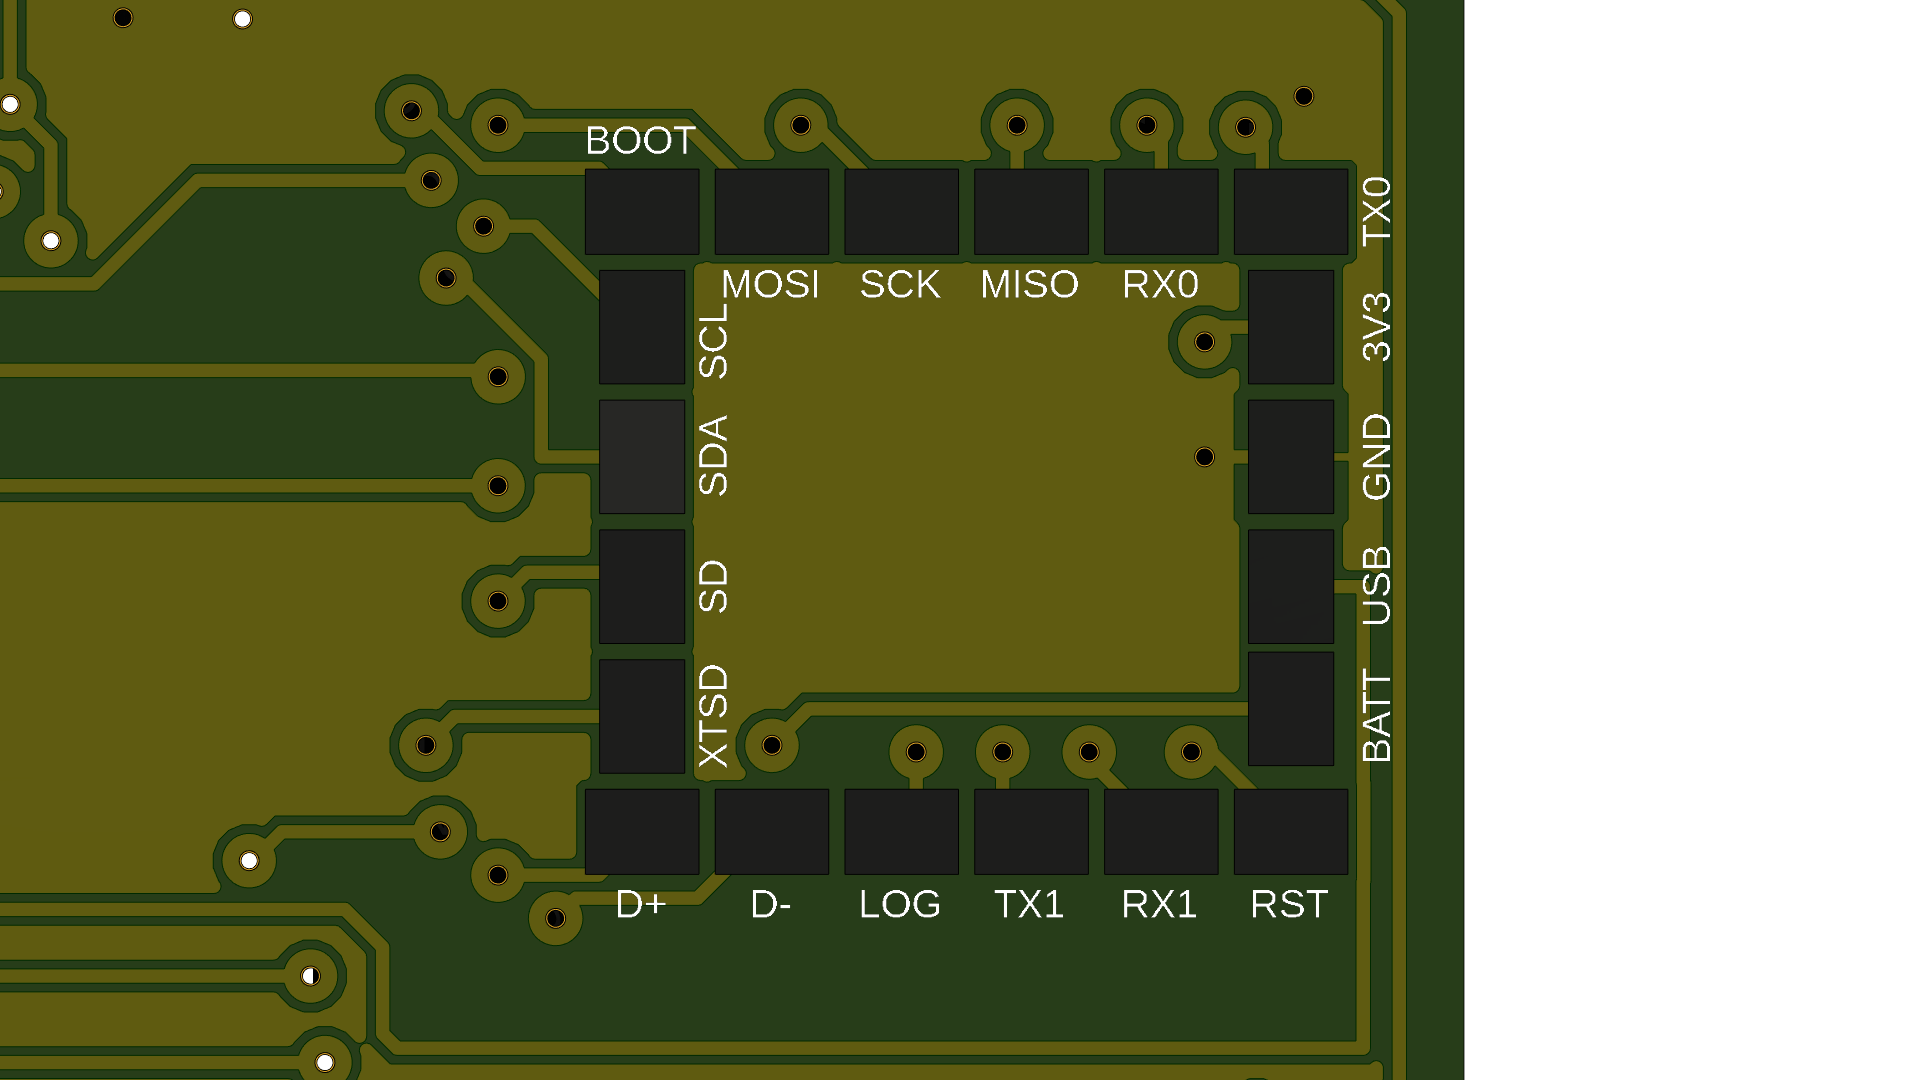
\includegraphics[width=0.85\textwidth]{board_back.png}};
        \node[annotation] at (-2.25,2.32) {1};
        \node[annotation] at (-1.30,2.32) {2};
        \node[annotation] at (-0.4,2.32) {3};
        \node[annotation] at (0.5,2.32) {4};
        \node[annotation] at (1.4,2.32) {5};
        \node[annotation] at (2.35,2.32) {6};
        \node[annotation] at (2.35,1.5) {7};
        \node[annotation] at (2.35,0.6) {8};
        \node[annotation] at (2.35,-0.3) {9};
        \node[annotation] at (2.35,-1.2) {10};
        \node[annotation] at (2.35,-2.07) {11};
        \node[annotation] at (1.43,-2.07) {12};
        \node[annotation] at (0.5,-2.07) {13};
        \node[annotation] at (-0.4,-2.07) {14};
        \node[annotation] at (-1.3,-2.07) {15};
        \node[annotation] at (-2.25,-2.07) {16};
        \node[annotation] at (-2.25,-1.2) {17};
        \node[annotation] at (-2.25,-0.3) {18};
        \node[annotation] at (-2.25,0.6) {19};
        \node[annotation] at (-2.25,1.5) {20};
    \end{tikzpicture}
    \caption{PCB interface pinout}
    \label{fig:pcb_interface_pinout}
\end{figure}

\begin{multicols}{2}
\customTable
{l l l l}
{Pad & Name & Bus & Type}
{
    1 & Boot Select & \acs{GPIO} & Input \\
    2 & \acs{MOSI} & \acs{SPI} & Output \\
    3 & \acs{SCK}  & \acs{SPI} & Clock \\
    4 & \acs{MISO} & \acs{SPI} & Input \\
    5 & \acs{RX}0  & \acs{UART}0 & Input \\
    6 & \acs{TX}0 & \acs{UART}0 & Output \\
    7 & 3V3 & & Power \\
    8 & GND & & Power \\
    9 & VUSB & & Power \\
    10 & VBATT & & Power \\
}
{PCB interface pinout}
{tab:pcb_interface_pinout}

\customTable
{l l l l}
{Pad & Name & Bus & Type}
{
    11 & Reset & \acs{GPIO} & Input \\
    12 & \acs{RX}1 & \acs{UART}1 & Input \\
    13 & \acs{TX}1 & \acs{UART}1 & Output \\
    14 & Log & \acs{GPIO} & Input \\
    15 & D- & \acs{USB} & Data \\
    16 & D+ & \acs{USB} & Data \\
    17 & XTSD \acs{CS} & \acs{SPI} & Output \\
    18 & \acs{microSD} \acs{CS} & \acs{SPI} & Output \\
    19 & \acs{SDA} & \acs{I2C} & Data \\
    20 & \acs{SCL} & \acs{I2C} & Clock \\ 
}
{PCB interface pinout}
{tab:pcb_interface_pinout}
\end{multicols}{2}

\vskip 1em

\warning{Incorrect connections to the PCB interface may cause permanent damage.  
This interface should only be used by an experienced engineer with the appropriate carrier board.}

\clearpage

\subsection{Housing}

The housing components are annotated in \Fref{fig:enclosure_labeled}.  
A detailed mechanical drawing describing the housing dimensions is available in the Appendix. % TODO: Create reference.

\vskip 2em

% \begin{figure}[H]
%     \centering
%     \begin{tikzpicture}[annotation/.style={circle, draw=black, fill=white, very thick, minimum size=7mm}]
%         \node at (0,0) {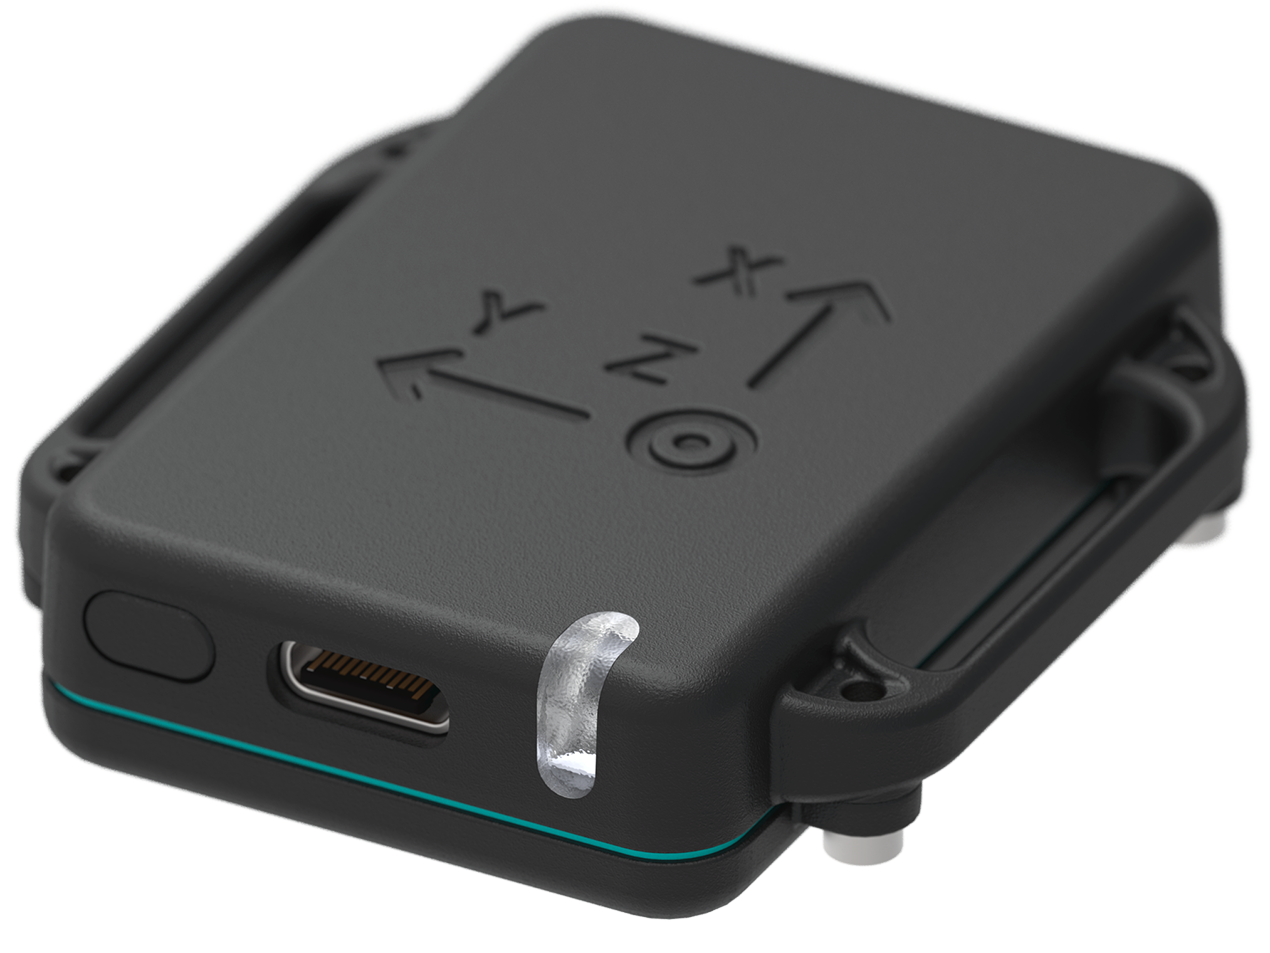
\includegraphics[width=0.8\textwidth]{Images/housing.png}};
%         \node[annotation] at (-5.6,-2) {\ref{itm:housing1}};
%         \node[annotation] at (-3.7,-2.55) {\ref{itm:housing2}};
%         \node[annotation] at (-1.2,-3.2) {\ref{itm:housing3}};
%     \end{tikzpicture}
%     \caption{Housing}
%     \label{fig:housing}
% \end{figure}

% \vskip 1em

% \begin{enumerate}
%     \item \label{itm:housing1} Power button
%     \item \label{itm:housing2} \acs{USB}-C connector
%     \item \label{itm:housing3} \acs{LED}
% \end{enumerate}

\begin{figure}[h!]
    \centering
    \subfloat[Sealed enclosure ready for deployment]{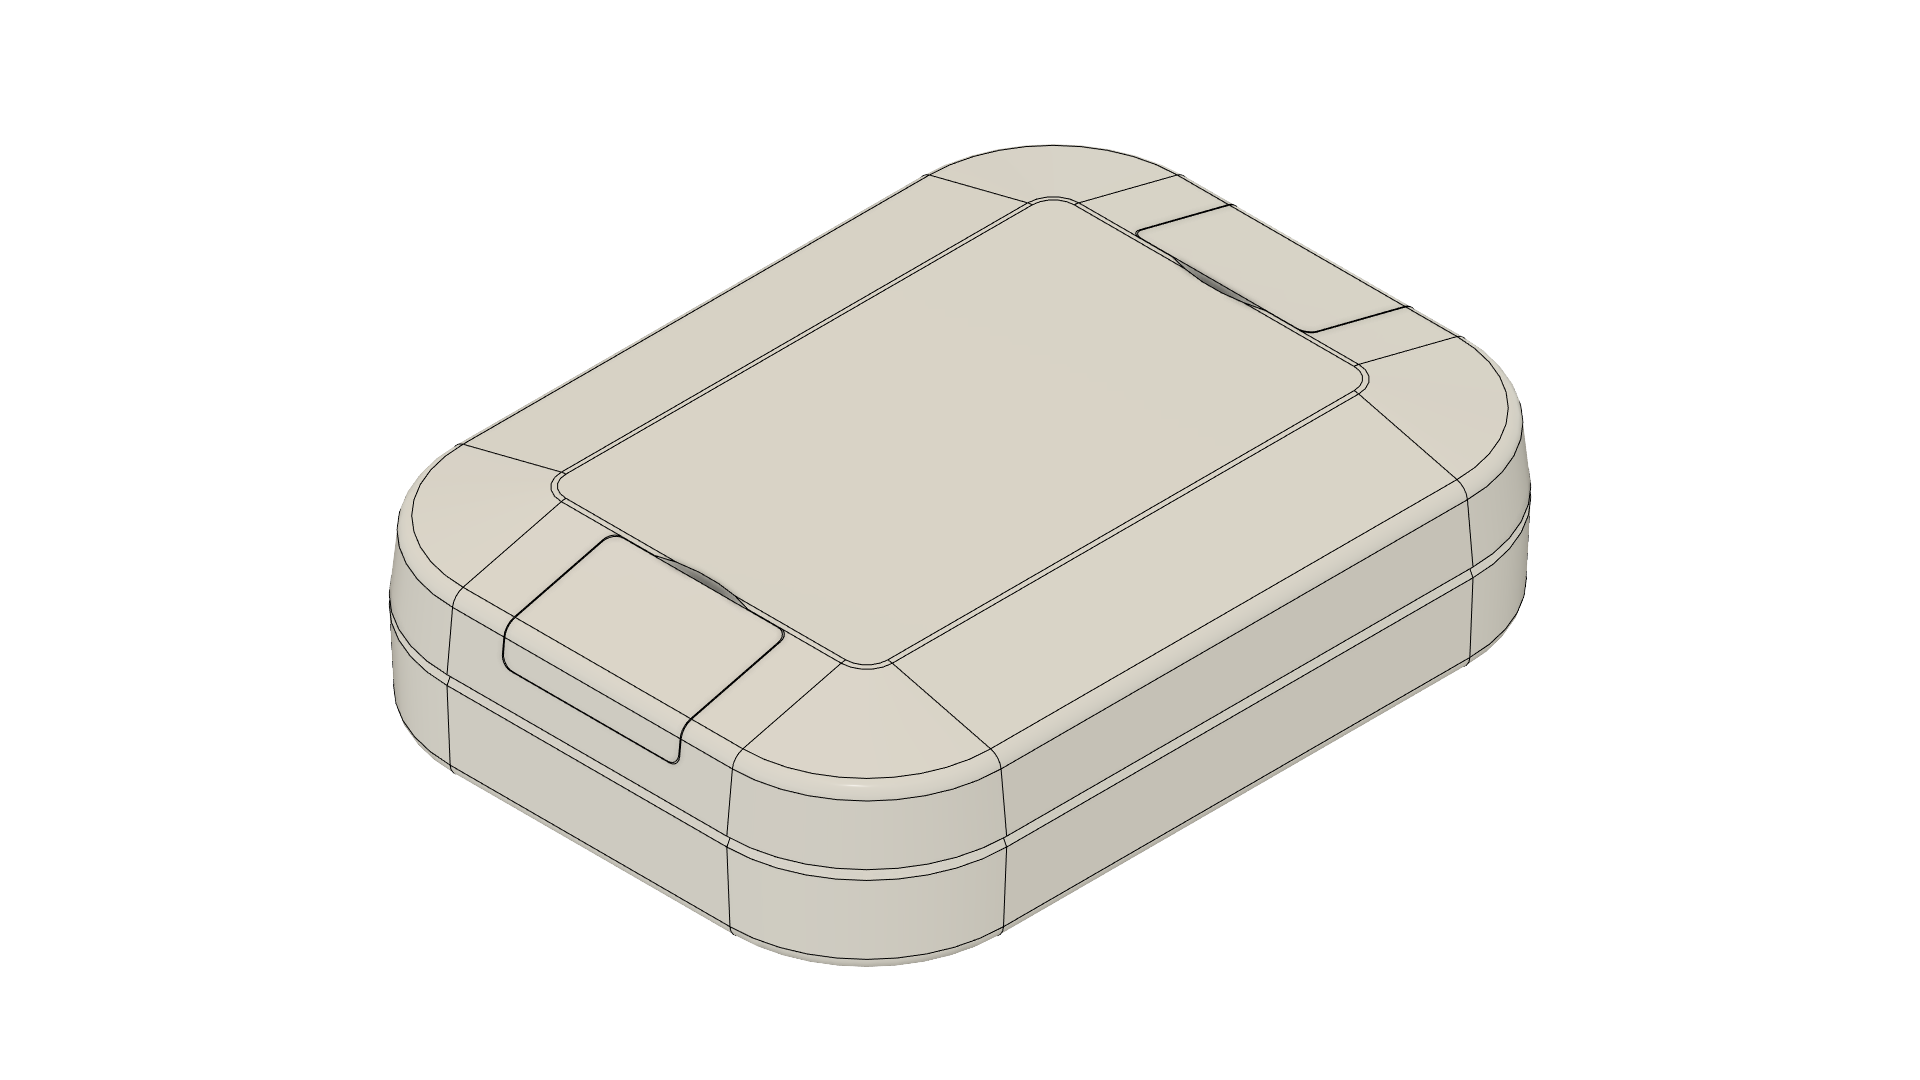
\includegraphics[height=3in]{thetis_enclosure.png}} \vskip6ex
    \subfloat[Enclosure with the top removed]{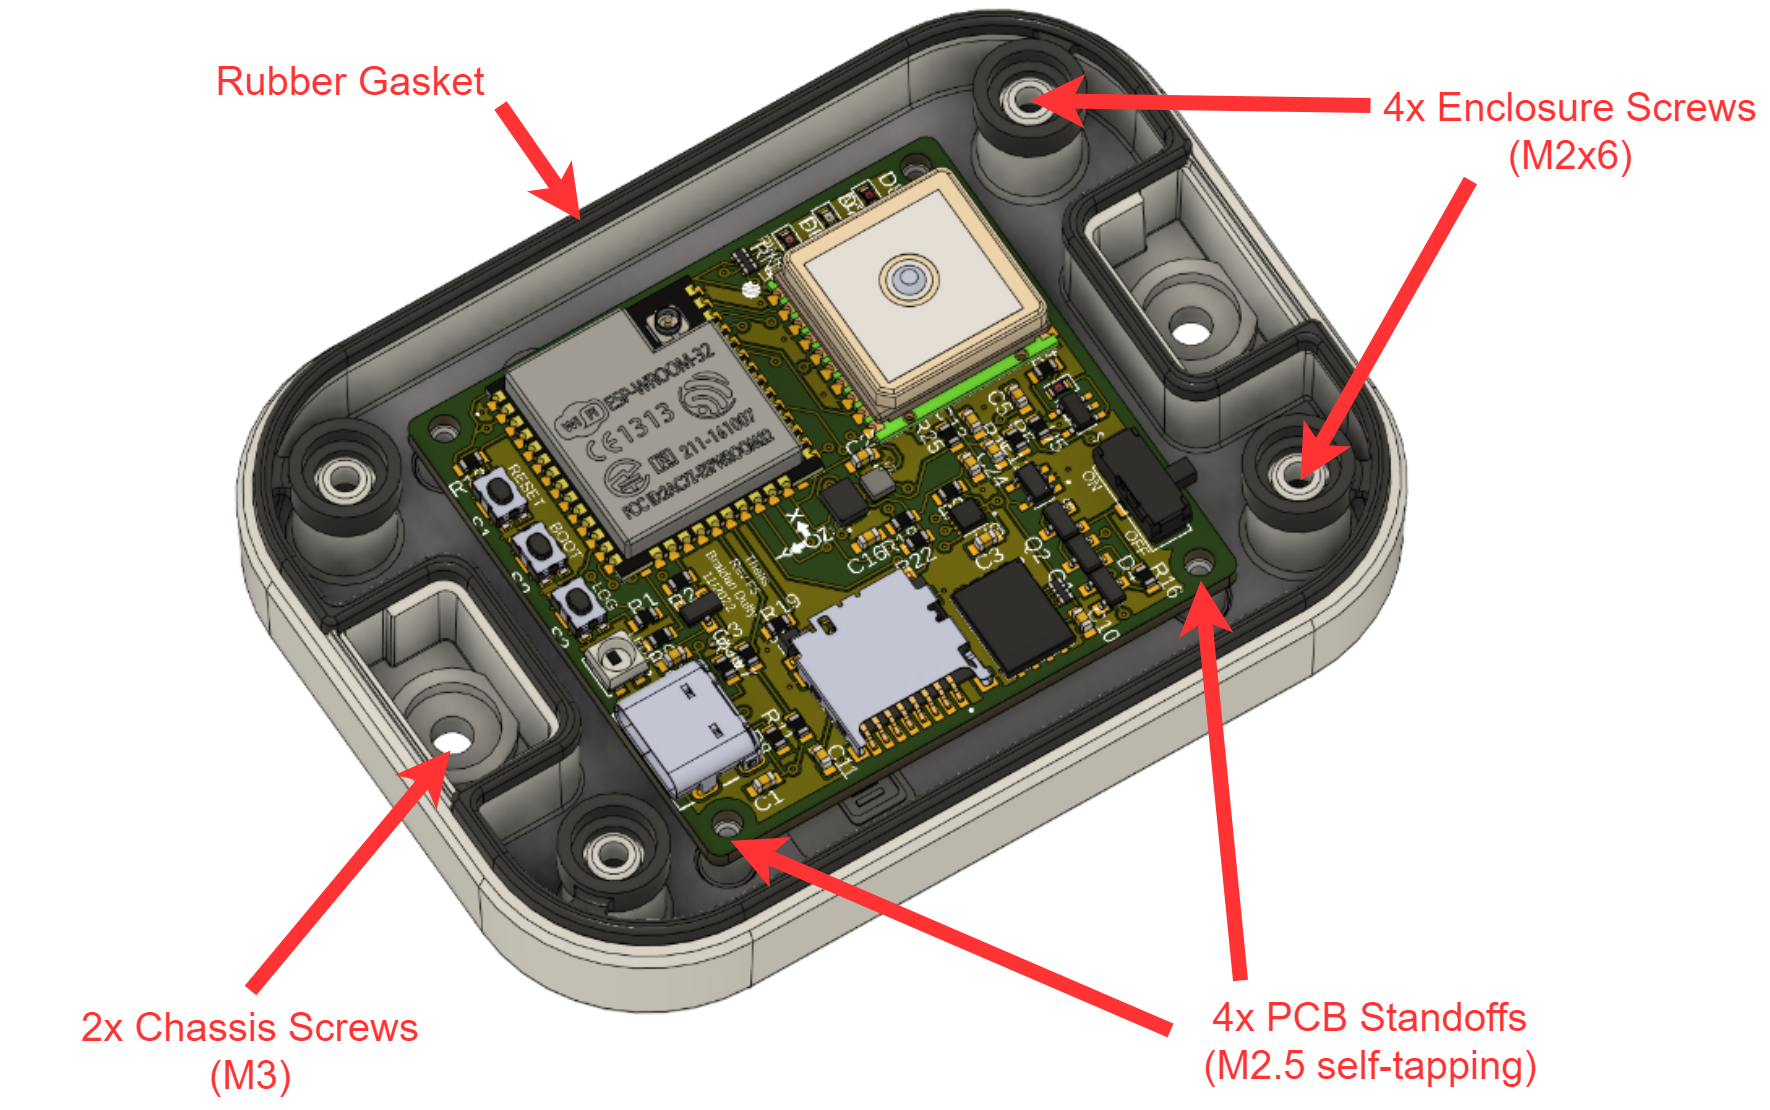
\includegraphics[width=\textwidth]{thetis_enclosure_labeled.png}}
    \caption{Thetis enclosure}
    \labfig{enclosure_labeled}
\end{figure}

\subsubsection{\acs{IP67} rating}

The \ac{IP67} rating is an international standard that describes the ability of the housing to protect against the ingress of solid particles and water.  
The first digit, 6 indicates complete protection against dust and solid particles.  
The second digit, 7 indicates protection from water for a maximum depth of 1 meter for up to 30 minutes.

In practical terms, this means that the housing can be used outdoors in all weather conditions and that it will survive accidental or temporary submersion in water.  
The housing has been tested in submerged applications up to 20-feet for 30 minutes, however typical applications \underline{should not} exceed the IP rating.
Always check that the gasket is in place, the 4 enclosure screws are suitably tightened, and the case is not cracked.

\vskip 1em

\warning{Over-torquing the enclosure screws may result in the plastic around them cracking.
The enclosure screws should be finger tight with an extra quarter turn.
Additionally, all four screws must be present for the case to be sealed - any less and the enclosure will leak when submerged!}

\clearpage
